%# -*- coding: utf-8-unix -*-
%%==================================================
%% chapter01.tex for SJTU Master Thesis
%%==================================================

%\bibliographystyle{sjtu2}%[此处用于每章都生产参考文献]
\chapter{前言}
\label{chap:preli}


\section{机器学习}

机器学习是一种赋予计算机学习能力,并让它完成直接编程无法完成的功能的方法。它研究的主要内容是关于在计算机上从经验数据中产生模型(model)的算法。我们为计算机提供经验数据,计算机使用这些数据产生模型,然后利用模型对同类数据进行推测。机器学习的产生与模仿人类思考模式的过程相关。人类通过学习,积累知识经验,归纳生活规律。当人类遇到未知的问题或对未来进行推测时,就可以使用这些经验生活规律进行推测。机器学习中的“训练”和“预测”即对应人类的“归纳”和“推测”。

机器学习的理论基础覆盖了各个学科,包括概率论、线性代数、数理统计等。同时,机器学习也是一种解决问题的工具,可以和其他领域的各种技术相结合,形成众多的交叉学科,包括数据挖掘、语音识别技术、计算机视觉、语音识别技术、自然语言处理等。数据挖掘领域中,机器学习算法拥有处理海量数据的能力,计算机可以从大量的数据中发现有价值的数据;计算机视觉领域中,机器学习技术与图像处理技术相结合,图像处理技术将待处理的图像转换为适合机器学习算法的输入的形式,然后机器学习算法再从图像中进行各种操作,该领域的典型应用有手写识别技术等;语音识别技术领域内,音频处理技术和机器学习技术相结合,机器学习算法那分析音频信号,然后将音频信号翻译成语言,例如苹果公司的Siri和微软的Cortana等;自然语言处理领域中,研究者们试图使用词法分析、语法分析等编译相关的知识,让计算机理解人类的语言,是机器学习分类中备受瞩目的一个分支。

机器学习的算法种类五花八门。其中最为重要的几类算法主要如下所示:

\begin{enumerate}
	\item [(1)] \textbf{回归算法(Regression)}:回归类算法那的代表是线性回归(Linear Regression)算法和逻辑回归(Logistic Regression)算法。线性回归算法的主要思想是最小二乘法,主要目标是寻找一条可以最好地拟合训练数据的直线。逻辑回归与线性回归原理类似,但线性回归的目标是对未知的数值结果进行预测,而逻辑回归的目标是对未知的二分类问题进行判断。
	\item [(2)] \textbf{神经网络(Neural Networks, NN)}:神经网络算法是一种利用计算机模拟大脑的思考过程的算法。神经网络算法的结构有很多层,它可以对数据进行分解,由每层的大量“神经元”结构处理数据,并把处理后的数据送给下一层神经元。每一个神经元都是一个微型的逻辑回归模型,众多的神经元层层叠加,可以处理普通的回归模型难以处理的、非常复杂的分类问题。神经网络有很多种经典类型,例如多层感知机MLP(Multi-layer Perceptron)和卷积神经网络CNN(Convolutional Neural Network)等。神经网络的一个典型的应用就是手写数字识别问题(MNIST)。
	\item [(3)] \textbf{支持向量机(Support Vector Machine, SVM)}:SVM算法也是一种非常经典的判别式算法,是逻辑回归的优化版,可以更好地划分分类线。核(Kernel)函数是SVM的一个重点。与不同的核函数结合,SVM可以在低维空间表达出高维空间的分类线,在保留原本计算复杂性的条件下大大增强了分类的准确度。
	\item [(4)] \textbf{聚类算法(Clustering Algorithm)}:前三类算法都称为监督算法,使用的基本条件是训练数据必须带有标签,在训练后可以对同类型未标签的数据进行预测。而聚类算法是应用于无标签数据集上的算法,它可以计算数据群体中相互之间的距离,并根据距离的大小将数据划分为多个类别。典型的聚类算法是K-Means算法。
	\item[(5)] \textbf{降维算法}:降维算法的主要作用是压缩数据的维度,以提升其他算法在该数据集上的计算效率,是一种辅助型算法。降维算法可以在多特征的数据中提取主要特征,除去数据中的冗余信息,在最大程度保留原本信息的前提下,降低计算复杂度。最具有代表性的降维算法是主成分分析PCA(Principal Component Analysis)。
	\item[(6)] \textbf{推荐算法}:推荐算法在电商平台上的应用很广,可以根据用户的购买信息和浏览记录,自动推荐他们可能产生兴趣的商品,从而增加商品的售出率,提升店家的经济效益。最有名的推荐算法是协同过滤(Collaborative Filtering)算法。
\end{enumerate}

除了上述列出的算法以外,机器学习领域还有诸如用于决策的增强学习(Reinforcement Learning)、多隐藏层神经网络的深度学习(Deep Learning)等大型分支。机器学习是目前最火热的计算机科学领域之一。从AlphaGo到智能车自动驾驶,从谷歌识图到微软小冰,机器学习的实践应用也屡屡让世界惊叹。



\section{网络诈骗中的分类算法}

网络诈骗有多种类型,例如网页诈骗 \cite{Spirin:2012}、邮件诈骗 \cite{Castillo:2007}、远程通信诈骗 \cite{Yao:2017}和概念诈骗 \cite{Jindal:2008}等。水军检测问题属于概念诈骗领域。面对这类问题,早期研究者们热衷于使用NLP和数据挖掘技术对评论中表达出的各种观点进行分类和总结。后来他们试图优化文本分析方法,Chen等人 \parencite{Chen:2013}提出了基于语义分析的方法,用拆句子工具将评论内容拆分为一个个单词,并通过计算不同评论内容拆分后单词的相似数来衡量语义的相似程度。他们也尝试了使用非监督学习的方法进行检测,但效果并不是很好。Shojaee等人 \parencite{Shojaee:2013}认为关注水军评论内容的词法特征和语法特点很关键。由于水军们试图模仿正常评论的内容来隐藏水军评论,所以他们的写作风格和用词风格一直在变化。因此,只纠结于词法和语法形式是事倍功半的。但是如果从文体形式出发来考虑的话,就可以辨别出水军评论的相似性,进一步找到那些虚假评论。他们提取出这些特征后使用经典的分类算法和进行检测。

抛开NLP方法,在机器学习方法的帮助下,水军检测问题可以被视为二分类问题或排名问题。其中的关键部分便是特征的选取和模型的选取。可以在水军检测中应用的经典机器学习分类算法有很多:Ott等人 \parencite{Ott:2011}提出了SVM和单词条/双词条文本分析的结合,Chen等人 \parencite{CHEN:2009}提出了朴素贝叶斯NB(Naive Bayes)在文本分类问题中的应用。也有许多研究者在经典方法的基础上进行了改进,并提出了新的方法。Li等人 \parencite{Li:2014}提出了PU(Positive-Unlabeled)学习方法。他们认为在网络平台的过滤系统作用下,那些被过滤系统过滤掉的评论一定是虚假评论,然而被过滤系统判定为正常的评论中却还混有大量的虚假评论。故PU学习适用的数据集是那些只部分标记了一种类型数据,其他数据视为未标记数据的情况。他们还与大众点评公司合作,取得了珍贵的数据,在此基础上提出了新颖的模型。Chino等人 \parencite{Chino:2017}利用用户发布评论的时间间隔和评论内容量特征,训练了一个对数分布模型来拟合大众的特征分布情况,然后找到那些与主流分布隔离开来的点,将这些点视作可疑用户。这种寻找与大众情况相异用户的思路非常有效。Chen等人 \parencite{Chen:2017}提出了一个利用目标排名变动情况来寻找可疑用户的模型。如果目标短时间内在排行榜上发生了大幅震荡——排名迅速上升几天后又迅速下跌——那目标很可能雇佣了水军帮助他增长排名。不仅如此,他们还利用这一点进一步分析,成功捕捉到了水军团队。




\section{随机过程}

随机过程(Stochastic Process)是一系列随机事件动态关系的定量描述。数学上的定义如下所示:

\begin{defn}
	设对每一个$t \in T$,$X(t,\omega)$是一个随机变量,称随机变量族 $X_T = \{X(t,\omega), t \in T\}$为一个随机过程,该函数称为随机函数,其中$T \in \Re$称为指标集, $\Re$是实数集, $\omega \in \Omega$, $\Omega$为样本空间。用一个映射关系来表示 $X_T$则有:
	\begin{equation}
		X(t,\omega):T \times \Omega \rightarrow \Re
	\end{equation}
\end{defn}

根据定义,$X(t,\omega)$是一个定义在$T \times \Omega$上的二元单值函数,其中$T \times \Omega$表示二者的笛卡尔积。如果参数 $t \in T$取时间的话,则该函数是一个描述样本随时间变化的随机过程。这种情况下,通常称$X_t (t \in T)$为随机状态,$X_T = \{X(t,\omega), t \in T\}$是$X_t$可能取值的全体集合,称为状态空间。

马尔可夫过程(Markov Process)是本研究中主要关注的一种随机过程。一个随机过程若已知某个现在状态,其将来状态不受到过去状态的影响,即各个状态相互独立,则该过程称为马尔可夫过程。准确的数学定义如下:

\begin{defn}
	若随机过程$\{X_T, t \in T\}$,状态空间为$E$,对任意$t_1 < t_2 < \cdots < t_n < t$和任意$x_i, 1 \leq i \leq n, x \in E$,随机变量$X(t)$在已知变量$X(t_1) = x_1, \cdots X(t_n) = x_n$之下的条件分布函数只与$X(t_n) = x_n$有关,而与$X(t_1) = x_1, \cdots X(t_{n-1}) = x_{n-1}$无关,即:
	\begin{equation}
		P\{X(t) \leq x | X(t_n) = x_n, \cdots , X(t_1) = x_1\} = P\{X(t) \leq x | X(t_n) = x_n\}
	\end{equation}
	则称该过程为马尔可夫过程。
\end{defn}

对于马尔可夫过程$X_T = \{X_t, t \in T \}$,当状态空间$E = \{1,2,3,\cdots\}$为可列无限集或有限集时,该过程通常称为马尔可夫链(Markov Chain)。




\section{隐马尔可夫模型}

隐马尔可夫模型HMM(Hidden Markov Model)是一种用单一离散随机变量描述过程状态的时序概率图模型。如图~\ref{fig:hmm},HMM可以用图来表示各个变量之间的关联。HMM有两个状态:观测态(图中$X_1 \cdots X_n$)和隐藏态(图中$Y_1 \cdots Y_n$)。隐藏态变量$Y_i$形成序列结构,然后每个隐藏态变量$Y_i$生成一个观测态变量$X_i$。在初始化时,HMM有一个初始状态概率(Initial State Probability)来决定由哪种隐藏态开始构建序列。之后每次出现一个新状态,隐藏态序列就增加一个变量,并且新的隐藏态变量的值受到前一个隐藏态变量的影响,这个影响遵循一个特定的转移概率(Transition Probability)。每个隐藏态变量生成观测态变量的过程也遵循一个特定的输出概率(Emission Probability)。为了保证序列本身和各种概率的的合理性,HMM遵循两个重要的假设:
\begin{enumerate*}		
	\item[(1)] 每一个隐藏态变量的生成都只依赖于它之前的那一个隐藏态变量;
	\item[(2)] 每一个观测态变量的生成都只依赖于它对应的那个隐藏态变量。
\end{enumerate*}
这两个假设称为马尔可夫假设,在大量的实践中被广泛认可。它们在不对结果产生重大影响的前提下大大简化了模型的计算复杂度。

\begin{figure}[htbp]
	\centering
	\begin{minipage}[htbp]{\textwidth}
		\centering
		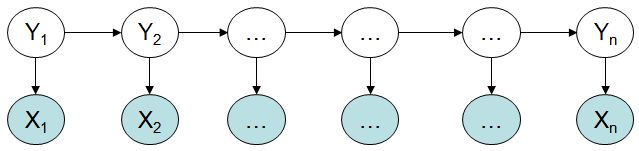
\includegraphics[width=10cm]{preli-1.jpg}
		\caption[HMM示例图]
		{HMM示例图\label{fig:hmm}}		
	\end{minipage}     
\end{figure}


在HMM的应用实例中,观测态相当于观测现象的数学表现,隐藏态相当于真实情况的数学表现,而整个模型相当于根据观测情况对真实情况进行的推理。这个推理过程可以用数学语言表示为$P(X_i |Y_i)$,这就是HMM的输出概率。另一方面,当前的真实情况应该与其上一个真实状态相关,即应该存在这样一个分布$P(Y_i | Y_{i-1})$,这就是HMM的转移概率。并且它们也保证了转移概率和输出概率的合理性。


由于HMM中的隐藏态是有限的离散量,所以通常我们把HMM中所有的转移概率写成矩阵的形式。若HMM中有$k$种隐藏态,则对应转移概率矩阵的大小为$k \times k$,其中第$m$行,第$n$列的值就是$P(Y_i = n | Y_{i-1} = m)$,即给定隐藏态为m时,下一时刻转换到状态n的概率。而对于输出概率的表示,由于HMM的观测态既可以是离散量也可以是连续量,故我们需要分类讨论。当观测态是有限的离散量,且观测态共有$l$种时,输出概率也可以用一个大小为$k \times l$的矩阵表示,其中第$m$行,第$n$列的值就是$P(X_i = n | Y_{i-1} = m)$,即对应隐藏态为$m$时,该观测态为$n$的概率。而对于观测态连续的情况,若观测态属于某一种连续分布,则若有$k$个隐藏态,输出概率就是一个包含$k$个不同参数的该连续分布的分布函数的集合。


综上所述,一个确定的HMM模型由三个参数定义:初始状态概率、转移概率和输出概率。

用HMM解决的问题主要有三种类型:

\begin{enumerate}		
	\item[(1)] \textbf{参数估计}:给定一个观测序列,计算一组参数(三个概率)使该观测序列出现的可能性最大;
	\item[(2)] \textbf{由观测态序列确定隐藏态序列(解码问题)}:已知HMM模型,给定一个观测序列,求解最可能的隐藏序列;
	\item[(3)] \textbf{求解观测序列出现的概率}:已知HMM模型,给定一个观测序列,计算该序列出现的概率。
\end{enumerate}

参数估计问题就是HMM的训练问题。Rabiner在1989年提出了一种名为\emph{Baum-Welch}\cite{Rabiner:1989}的EM(Expectation-Modification)算法,利用极大似然估计方法来训练HMM参数,现在已经成为了该问题的普遍解决策略。由观测态序列确定隐藏态序列的问题在语音识别领域也称作解码问题,目标是在给定观测序列的情况下寻找概率最高的隐藏序列。Forney在1973年提出来了解决这种问题的\emph{Viterbi}\cite{Forney:1973}算法。计算观测序列概率的问题是计算特定HMM生成特定观测序列的概率。换句话说,这个问题可以用来计算观测序列和给定模型的关联程度。


在一些前人的工作中,研究者们提出了关于将HMM利用在水军检测任务中的可能性的研究。Malmgren等人 \parencite{Malmgren:2009}提出了一个基础的双链HMM模型,并提出了一个高效的算法,使用现有的数据训练这个模型。Washha等人\parencite{WASHHA:2017}也证明了在水军检测模型中使用HMM的可能性。Li等人\parencite{Li:2017}提出了一个LHMM(Labeled Hidden Markov Model)模型,并将该模型与时间间隔特征结合,在一个大众点评数据集中进行水军检测,并取得了优秀的成果。


